\documentclass[10pt]{beamer}
\usetheme{jambro}

\title[]{Pensamento Econômico Contemporâneo - Teoria Geral e emergência da Macroeconomia moderna}
\author[]{Paulo Victor da Fonseca}
\date{}

\hypersetup{
    colorlinks = true,
    urlcolor = teal,
    linkcolor = teal    
}
\usepackage[portuguese]{babel}
\usepackage{subfig}
\usepackage{emoji}

\begin{document}

\begin{frame}[plain]
    \titlepage{
        \begin{center}
            \begin{minipage}{0.8\textwidth}
                \centering
            \end{minipage}
        \end{center}}
\end{frame}

\begin{frame}{Sumário}
    \tableofcontents
\end{frame}

\section{Mercado de trabalho: a análise de Keynes}
\begin{frame}{Introdução}
    \begin{itemize}
        \item Modelo clássico: hipóteses de competição perfeita no mercado de trabalho e flexibilidade perfeita de salários e preços garantem equilíbrio de pleno emprego
        \bigskip
        \item Keynes: funcionamento do mercado de trabalho nem sempre assegura condição de \textcolor{blue}{market clearing} (condição de equilíbrio entre demanda e oferta sem que exista uma situação de excesso de oferta ou demanda)
        \bigskip
        \item \textcolor{blue}{Desemprego involuntário} é, provavelmente, uma característica dos mercados de trabalho se há rigidez de salários nominais
        \bigskip
        \item Para Keynes, ainda, a flexibilidade de salários nominais não seria suficiente para gerar forças que assegurem que a economia retorne para equilíbrio de pleno emprego
        \bigskip
        \item Analisaremos, agora, cada um destes casos
    \end{itemize}
\end{frame}

\subsection{Rigidez dos salários nominais}
\begin{frame}{Mercado de trabalho: rigidez de salários nominais}
    \begin{itemize}
        \item Teoria Geral: inicialmente assume que salários nominais são `constantes' para `facilitar a exposição'
        \bigskip
        \NB{``O fato de os sal\'{a}rios nominais e de outros aspectos estarem ou n\~{a}o sujeitos a varia\c{c}\~{a}o em nada altera a natureza do racioc\'{i}nio'' 
        
        \begin{flushright}
        (Keynes, 1936)
        \end{flushright}}
        \bigskip
        \item Qual o impacto de um choque adverso de DA sobre o produto agregado real e o nível de emprego no caso de rigidez nominal de salários?
    \end{itemize}
\end{frame}

\begin{frame}{Mercado de trabalho: rigidez de salários nominais}
    \begin{figure}
        \centering
        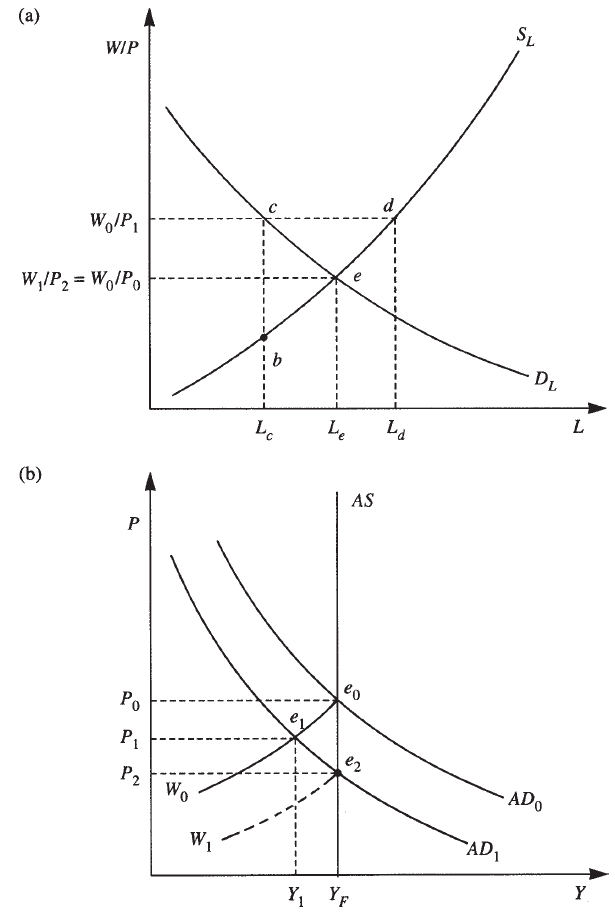
\includegraphics[width=0.3\textwidth]{./figures/aula5_fig1.PNG}
        \caption{Desemprego involuntário em Keynes. Fonte: Snowdon e Vane (2005).}
        \label{fig1}
    \end{figure}
\end{frame}

\begin{frame}{Mercado de trabalho: rigidez de salários nominais}
    \begin{itemize}
        \item Economia inicialmente em equilíbrio de pleno emprego
        \bigskip
        \item Choque adverso de DA desloca a curva de demanda agregada de $AD_0$ para $AD_1$
        \bigskip
        \item Com preços são flexíveis mas salários nominais rígidos, a economia se move do ponto $e_0$ para $e_1$
        \bigskip
        \item Rigidez nominal dos salários: a curva de oferta agregada torna-se $W_0AS$
        \bigskip
        \item Com a queda do nível de preços para $P_1$ e salários nominais permanecendo em $W_0$, o salário real aumenta para $W_0/P_1$
        \bigskip
        \item A este novo valor de salário real, a oferta de trabalho $L_d$ excede a demanda de trabalho por parte das firmas $L_c$ e, portanto, um \textcolor{blue}{desemprego involuntário} de magnitude $cd$ emerge
    \end{itemize}
\end{frame}

\begin{frame}{Mercado de trabalho: rigidez de salários nominais}
    \NB{Existem desempregados involunt\'{a}rios quando, no caso de uma ligeira eleva\c{c}\~{a}o dos pre\c{c}os dos bens de consumo de assalariados relativamente aos sal\'{a}rios nominais, tanto a oferta agregada de m\~{a}o-de-obra disposta a trabalhar pelo sal\'{a}rio nominal corrente quanto a procura agregada da mesma ao dito sal\'{a}rio s\~{a}o maiores que o volume de emprego existente.
        \begin{flushright}
            (Keynes, 1936)
        \end{flushright}}    
\end{frame}

\begin{frame}{Mercado de trabalho: rigidez de salários nominais}
    \begin{itemize}
        \item Dado que uma quantidade $L_e - L_c$ de desempregados involuntários estão dispostos a trabalhar a um salário real de equilíbrio $W_0/P_0$, uma queda no salário real de $W_0/P_1$ para $W_0/P_0$ é aceitável para eles, como indicado pela curva de oferta de trabalho entre $b$ e $e$
        \bigskip
        \item Uma queda no salário real também induziria as firmas maximizadoras de lucro a demandarem mais trabalho
    \end{itemize}
\end{frame}

\begin{frame}{Mercado de trabalho: rigidez de salários nominais}
    \begin{itemize}
        \item Mas como o salário real pode ser reduzido?
        \bigskip
        \begin{enumerate}
            \item Ou os salários nominais devem cair em relação ao nível de preços
            \bigskip
            \item Ou o nível de preços deve subir em relação ao salário nominal
        \end{enumerate}
        \bigskip
        \item Keynes dava preferência à segunda opção e advogava em favor de expansões de DA para exercer pressão sobre o nível de preços
        \bigskip
        \item Seriam necessárias políticas econômicas que deslocassem a curva de DA de $AD_1$ para $AD_0$
        \bigskip
        \item O aumento do nível de preços de $P_1$ para $P_0$ reduziria o salário real, restaurando o salário real de equilíbrio e eliminando o desemprego involuntário
    \end{itemize}
\end{frame}

\begin{frame}{Mercado de trabalho: rigidez de salários nominais}
    \begin{itemize}
        \item Keynes: política alternativa de corte de salários nominais rejeitada em termos práticos e teóricos
        \bigskip
        \item Em uma democracia caracterizada por processos de barganhas salariais decentralizadas, reduções salariais só aconteceriam, provavelmente, ``depois de lutas desastrosas e nocivas'', produzindo um resultado final que não seria justificável sob nenhum critério de ``justiça social ou de conveniência econômica''
        \bigskip
        \item Keynes também argumentava que trabalhadores não resistiriam a reduções do salário real causados por um aumento no nível real de preços, dado que isto manteria os salários reais relativos inalterados, o que é uma preocupação central da classe trabalhadora
    \end{itemize}
\end{frame}

\begin{frame}{Mercado de trabalho: rigidez de salários nominais}
    \begin{itemize}
        \item \hlight{Isso não implica que os trabalhadores sofram de ilusão monetária}
        \bigskip
        \item A resistência à cortes nos salários nominais e aceitação de redução nos salários reais via aumento generalizado do custo de vida tem a vantagem de preservar a estrutura existente de relatividades
        \bigskip
        \item Em qualquer um dos casos, dado que o trabalho só pode barganhar salários nominais e o nível de preços não é uma de suas variáveis de controle, não é possível que o trabalho consiga reduzir o salário real via revisões de barganhas salariais com empresários de maneira generalizada
    \end{itemize}
\end{frame}

\begin{frame}{Mercado de trabalho: rigidez de salários nominais}
    \begin{itemize}
        \item Keynes rejeitou a flexibilidade de preços e salários como um método confiável de restauração do equilíbrio também em termos teóricos
        \bigskip
        \item Uma flexibilização extrema dos salários nominais em uma economia monetária poderiam piorar a situação
    \end{itemize}
\end{frame}

\subsection{Flexibilidade dos salários nominais}
\begin{frame}{Mercado de trabalho: flexibilidade dos salários nominais}
    \begin{itemize}
        \item TG: Keynes demonstra que o canal pelo qual cortes no salário nominal eliminariam o desemprego involuntário seria, primariamente, via impacto que estes teriam sobre a taxa de juros
        \bigskip
        \item Se cortes salariais permitirem reduções subsequentes no nível de preços, o valor real da oferta de moeda aumenta o que, por sua vez, reduziria a taxa de juros e estimularia gastos com investimento
        \bigskip
        \item O corte salarial desloca a curva OA de $W_0AS$ para $W_1AS$, onde $W_1 < W_0$
        \bigskip
        \item A economia retornaria para o equilíbrio de pleno emprego no ponto $e_2$
        \bigskip
        \item Portanto, o mecanismo de preço permitiu um aumento de DA sem intervenções governamentais sob a forma de políticas de gerenciamento de demanda
    \end{itemize}
\end{frame}

\begin{frame}{Mercado de trabalho: flexibilidade dos salários nominais}
    \begin{itemize}
        \item Mecanismo conhecido como \textcolor{blue}{efeito Keynes}: estímulo indireto de DA (principalmente via gastos com investimento) induzido por queda na taxa de juros, que resulta de um aumento nos encaixes reais seguindo uma queda no nível geral de preços
        \bigskip
        \item Em termos do modelo IS-LM, o efeito Keynes é ilustrado por um deslocamento para a direita da curva LM
        \bigskip
        \item Como veremos mais adiante na disciplina, Keynes identificou duas razões para que o efeito Keynes poderia vir a não funcionar:
        \bigskip
        \begin{enumerate}
            \item \textcolor{blue}{Armadilha da liquidez}: impossibilita redução da taxa de juros
            \medskip
            \item Agenda de investimento inelástica com relação à taxa de juros: impossibilitaria a queda no nível de preços de estimular DA via variações na taxa de juros
        \end{enumerate}
        \bigskip
        \item Essas possíveis limitações de deflação como maneira de recuperação econômica seriam representadas por uma curva DA vertical abaixo do ponto $e_1$ (i.e., a economia não pode se deslocar de $e_1$ para $e_2$)
    \end{itemize}
\end{frame}

\begin{frame}{Mercado de trabalho: flexibilidade dos salários nominais}
    \begin{itemize}
        \item Keynes: políticas de redução de salários nominais para um dado nível de oferta de moeda poderiam, teoricamente, produzir os mesmos efeitos que uma política monetária expansionista para um dado nível de salário nominal
        \bigskip
        \item O que implica que a política monetária estaria sujeita às mesmas limitações que cortes salariais como uma maneira de assegurar o pleno emprego
        \bigskip
        \item No entanto, uma deflação de preços considerável teria, provavelmente, repercussões severas nas expectativas dos negócios, o que poderia levar a quedas subsequentes na DA
        \bigskip
        \item O impacto de uma deflação severa sobre a propensão marginal a consumir, via efeitos distributivos, também seria, provavelmente, adverso
    \end{itemize}
\end{frame}

\begin{frame}{Mercado de trabalho: flexibilidade dos salários nominais}
    \NB{Considerando a natureza humana e nossas institui\c{c}\~{o}es, somente uma pessoa insensata preferiria uma pol\'{i}tica de sal\'{a}rios flex\'{i}veis a uma pol\'{i}tica monet\'{a}ria el\'{a}stica, a n\~{a}o ser que pudesse invocar a favor da primeira vantagens imposs\'{i}veis de serem obtidas com a segunda [...] Supor que a pol\'{i}tica de sal\'{a}rios flex\'{i}veis seja um atributo normal e correlato de um sistema baseado, em seu conjunto, no princ\'{i}pio de \emph{laissez-faire} \'{e} o oposto \`{a} verdade
        \begin{flushright}
            (Keynes, 1936)
        \end{flushright}}
\end{frame}

\begin{frame}{Mercado de trabalho: flexibilidade dos salários nominais}
    \begin{itemize}
        \item Dadas as limitações do mecanismo de preços, para Keynes as autoridades deveriam tomar ações ativas para eliminar o desemprego involuntário
        \bigskip
        \item Caso não o fizessem, o sistema econômico poderia convergir para uma situação de equilíbrio estável de subemprego
        \bigskip
        \item Ou seja, haveria uma tendência para economias de mercado permanecerem em uma condição crônica de atividade subnormal por um período considerável ``sem tendência marcada para a recuperação ou o colapso completo''
    \end{itemize}
\end{frame}

\section{Lei de Say: a rejeição de Keynes}

\begin{frame}{Lei de Say: a rejeição de Keynes}
    \begin{itemize}
        \item Vimos, anteriormente, que quando a lei de mercados de Say é válida, políticas macroeconômicas de estímulo ou contração de DA são redundantes
        \bigskip
        \item Modelo clássico: a decisão de abster-se de consumo corrente é equivalente à decisão de consumir mais no futuro
        \bigskip
        \item Essa decisão, portanto, automaticamente implica que recursos deverão ser direcionados para a produção de bens de investimento que serão necessários para prover o fluxo de bens de consumo no futuro
        \bigskip
        \item Ou seja, um aumento na poupança automaticamente se torna um aumento nos gastos com investimento via ajustes na taxa de juros
        \bigskip
        \item \hlight{No modelo clássico, a poupança é apenas uma outra forma de consumo}
    \end{itemize}    
\end{frame}

\begin{frame}{Lei de Say: a rejeição de Keynes}
    \begin{itemize}
        \item Os princípios subjacentes à lei de Say estavam no centro das discussões de políticas  de recuperação econômica do período entre-guerras
        \bigskip
        \item Ralph Hawtrey: programas de obras públicas seriam inúteis dado que estes gastos iriam, simplesmente, deslocar uma quantidade equivalente de gastos privados - \textcolor{blue}{efeito crowding-out}
        \bigskip
        \item Esta visão, no entanto, só faz sentido em um contexto de uma economia operando no pleno emprego
    \end{itemize}
\end{frame}

\begin{frame}{Lei de Say: a rejeição de Keynes}
    \begin{itemize}
        \item Um dos objetivos da TG era fornecer uma refutação teórica da Lei de Say
        \bigskip
        \item No modelo de Keynes, emprego e produto agregados são determinados pelo princípio da demanda efetiva e, como vimos, o funcionamento dos mercados de trabalho não asseguram um equilíbrio de pleno empreg
        \bigskip
        \item A taxa de juros, por sua vez, é determinada nos mercados monetários $\neq$ modelo clássico (determinada pelas decisões de poupança e investimento)
        \bigskip
        \item Flutuações na eficiência marginal do investimento levariam a variações no produto real via efeito multiplicador e, como resultado, \hlight{poupança e investimento se equilibram via mudanças na renda agregada}
    \end{itemize}
\end{frame}

\begin{frame}{Lei de Say: a rejeição de Keynes}
    \begin{itemize}
        \item Keynes: qualquer desequilíbrio entre investimento planejado e poupança planejada leva a ajustes em quantidades, ao invés de ajustes via preços (taxa de juros)
        \bigskip
        \item Ao demonstrar as falhas inerentes na flexibilidade de preços e salários como um método de restaurar a economia ao equilíbrio de pleno emprego seguindo um choque negativo de demanda, Keynes efetivamente reverteu a lei de Say
        \bigskip
        \item No mundo de equilíbrio de subemprego de Keynes, \hlight{a demanda cria a oferta!}
    \end{itemize}
\end{frame}


\section{Keynes e a Teoria Quantitativa da Moeda}
\begin{frame}{Keynes e a TQM}
    \begin{itemize}
        \item Modelo clássico: choque monetário não tem efeito real - neutralidade da moeda
        \bigskip
        \item Dado que a quantidade de produto real é uma variável predeterminada pelo impacto combinado de um mercado de trabalho perfeitamente competitivo e pela lei de Say, qualquer variação na quantidade de moeda pode afetar, apenas, o nível de preços
        \bigskip
        \item Ao rejeitar a lei de Say e o modelo clássico de mercado de trabalho, a teoria de Keynes não assume que o produto real é predeterimando em seu nível de pleno emprego
    \end{itemize}
\end{frame}

\begin{frame}{Keynes e a TQM}
    \begin{itemize}
        \item No capítulo 21 da TG, Keynes discute as várias possibilidades:\medskip
        \begin{enumerate}
        \item \textcolor{blue}{Curva OA perfeitamente elástica}: mudança na demanda efetiva causada por um aumento na quantidade de moeda em circulação levará a um aumento no produto e emprego agregados sem ter efeitos sobre o nível de preços, até que o equilíbrio de pleno emprego seja atingido
        \medskip
        \item \textcolor{blue}{Situação `normal'}: aumento na demanda efetiva traduz-se, em parte, numa elevação da quantidade de emprego e, em parte, em elevação do nível de preços. Caso da Figura \ref{fig1} - expansões monetárias quando $Y < Y_F$ faz com que tanto o nível de preços quanto o produto aumentem
        \medskip
        \item \textcolor{blue}{Caso clássico:} quando o volume de produção corresponde ao de pleno emprego, o sistema econômico retorna para o caso clássico e, portanto, expansões monetárias só gerariam inflação
        \end{enumerate}
    \end{itemize}
\end{frame}

\begin{frame}{Keynes e a TQM}
    \begin{itemize}
        \item Uma complicação no modelo de Keynes é que o canal existente entre uma variação na quantidade de moeda e uma variação na demanda efetiva é indireto
        \bigskip
        \item Ele se dá via sua influência sobre a taxa de juros, investimento e o tamanho do multiplicador
        \bigskip
        \item Além disso, ao introduzir a teoria de preferência pela liquidez permite-se a possibilidade de que a função de demanda por moeda possa ser deslocada de maneira inesperada, causando flutuações na velocidade da moeda, isso, então, implica que variações em $M$ podem ser compensadas por variações em $V$ na direção contrária
        \bigskip
        \item Como $Y$ e $V$ não são mais variáveis constantes na obra de Keynes, fica claro que mudanças na quantidade de moeda em circulação $M$, pode levar a variações tanto em $P$ quanto em $V$ e $Y$
        \bigskip
        \item \hlight{A neutralidade da moeda não é mais assegurada!}
    \end{itemize}
\end{frame}

\section{Interpretações de Keynes}
\begin{frame}{Interpretações de Keynes}
    \begin{itemize}
        \item Coddington (1983) identificou três principais interpretações da Teoria Geral:
        \bigskip
        \begin{enumerate}
            \item A interpretação `hidráulica'.
            \bigskip
            \item A interpretação `fundamentalista'.
            \bigskip
            \item A abordagem modificada de equilíbrio geral.
        \end{enumerate}
    \end{itemize}
\end{frame}

\subsection{A interpretação hidráulica}
\begin{frame}{A interpretação hidráulica}
    \begin{itemize}
        \item A \textcolor{blue}{interpretação hidráulica} é a interpretação ortodoxa de Keynes.
        \bigskip
        \item Foi iniciada e inspirada pelos trabalhos de Hicks, Modigliani, Klein, Samuelson e Hansen.
        \bigskip
        \item O modelo IS-LM forma a espinha dorsal teórica desta abordagem e dominou o pensamento macroeconômico da síntese neoclássica dos anos 1950 e 1960.
    \end{itemize}
\end{frame}

\begin{frame}{A interpretação hidráulica}
    \begin{figure}
        \centering
        \subfloat[John Hicks (1904-1989)\label{fig3a}]{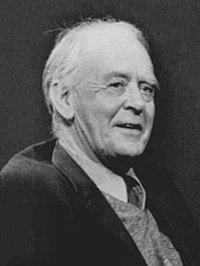
\includegraphics[width=0.22\textwidth]{./figures/aula5_fig2.jpg}} \quad
        \subfloat[Franco Modigliani (1918-2013)\label{fig3b}]{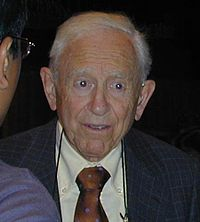
\includegraphics[width=0.26\textwidth]{./figures/aula5_fig3.jpg}} \quad
        \subfloat[Lawrence Klein (1920-2013)\label{fig3c}]{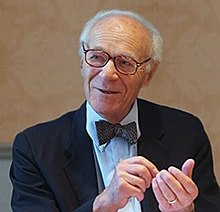
\includegraphics[width=0.3\textwidth]{./figures/aula5_fig8.jpg}}
        \caption{Economistas da interpretação `hidráulica'.}
        \label{fig3}
    \end{figure}
\end{frame}

\begin{frame}{A interpretação hidráulica}
    \begin{figure}
        \centering
        \subfloat[Paul Samuelson (1915-2009)\label{fig4a}]{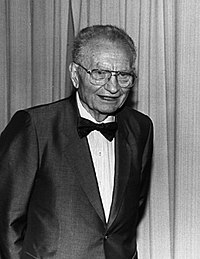
\includegraphics[width=0.3\textwidth]{./figures/aula5_fig4.jpg}} \quad
        \subfloat[Alvin Hansen (1887-1975)\label{fig4b}]{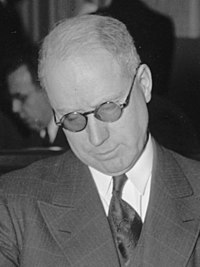
\includegraphics[width=0.3\textwidth]{./figures/aula5_fig5.jpg}}
        \caption{Economistas da interpretação `hidráulica'.}
        \label{fig4}
    \end{figure}
\end{frame}

\begin{frame}{A interpretação hidráulica}
    \begin{itemize}
        \item O livro texto de Paul Samuelson, publicado em 1948, foi de fundamental importância, popularizando Keynes com o \textcolor{blue}{diagrama da cruz Keynesiana}.
        \bigskip
        \item Com as contribuições de Franco Modigliani, a economia Keynesiana tornou-se \textcolor{blue}{a economia das rigidezes de preços e salários}.
        \bigskip
        \item O impacto desestabilizador de expectativas instáveis recebeu pouca atenção nessa abordagem.
        \bigskip
        \item Apesar de economistas como Modigliani e James Tobin terem trabalhado na microfundamentação do modelo de Keynes, uma das principais fraquezas da interpretação hidráulica é a falta de uma justificativa convincente para rigidezes salariais e de preços com base no comportamento racional dos agentes econômicos.
        \bigskip
        \item A abordagem hidráulica será estudada no próximo bloco da disciplina - \textcolor{blue}{Síntese neoclássica}, enquanto tentativas mais modernas de contornar as deficiências teóricas do modelo da síntese neoclássica serão objetos de estudo no bloco \textcolor{blue}{Novos-Keynesianos e o novo consenso macroeconômico}.
    \end{itemize}
\end{frame}

\subsection{A interpretação fundamentalista}
\begin{frame}{A interpretação fundamentalista}
    \begin{itemize}
        \item A \textcolor{blue}{interpretação fundamentalista} da Teoria Geral vê o trabalho de Keynes como um ataque frontal à ortodoxia neoclássica.
        \bigskip
        \item Fundamentalistas veem a influência de expectativas instáveis devido à incerteza como uma característica imprescindível em Keynes - capítulos 12 e 17 da Teoria Geral e ``The general theory of employment''.
        \bigskip
        \item Esta abordagem rejeita a interpretação hidráulica como uma ``bastardização'' da contribuição de Keynes.
        \bigskip
        \item As ideis e desenvolvimentos da \textcolor{blue}{escola pós-Keynesiana} não serão vistas neste curso.
    \end{itemize}
\end{frame}

\begin{frame}{A interpretação fundamentalista}
    \begin{figure}
        \centering
        \subfloat[George Shackle (1903-1992)\label{fig5a}]{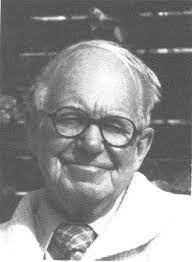
\includegraphics[width=0.3\textwidth]{./figures/aula5_fig6.jpeg}} \quad
        \subfloat[Joan Robinson (1903-1983)\label{fig5b}]{
\includegraphics[width=0.3\textwidth]{./figures/aula5_fig7.jpg}}
        \caption{Economistas pós-Keynesianos.}
        \label{fig5}
    \end{figure}
\end{frame}

\subsection{A abordagem modificada de equilíbrio geral}
\begin{frame}{A abordagem modificada de equilíbrio geral}
    \begin{itemize}
        \item Esta abordagem se inicia com a sugestão de Don Patinkin em 1956 de que \textcolor{blue}{a economia Keynesiana é a economia do desemprego de desequilíbrio e que o desemprego involuntário deve ser visto como um problema de desequilíbrio dinâmico.}
        \bigskip
        \item Na análise de Patinkin, o desemprego involuntário pode existir em uma economia perfeitamente competitiva com preços e salários flexíveis.
        \bigskip
        \item A ênfase dada à velocidade com que os mercados são capazes de absorver e corrigir choques desviou a atenção do grau de flexibilidade de preços e salários para problemas de coordenação.
        \bigskip
        \item Esta linha de pesquisa foi seguida por Clower (1956) e Leijonhufvud (1968), que desenvolveram uma abordagem de equilíbrio geral alternativa com características Walrasianas para incorporar os problemas de coordenação que emergem em uma economia de mercado operando sem a presença de um leiloeira Walrasiano ficcional.
    \end{itemize}
\end{frame}

\begin{frame}{A abordagem modificada de equilíbrio geral}
    \begin{itemize}
        \item A reinterpretação de Clower da Teoria Geral sugere que o objetivo de Keynes era abandonar a tradição de equilíbrio geral Walrasiana vigente na economia neoclássica.
        \bigskip
        \item No paradigma Walrasiano, todos os mercados estão continuamente em equilíbrio dada a presença de um leiloeiro ficcional.
        \bigskip
        \item A obra de Clower dá ênfase à natureza de desequilíbrio dinâmico de Keynes.
        \bigskip
        \item Para ele, o objetivo de Keynes era abandonar o mito do leiloeiro de forma a permitir um perfil de informação e dificuldades de coordenação intertemporal em economias reais.
        \bigskip
        \item Os declínios cumulativos no produto agregado, então, resultam de falhas de coordenação massivas à medida que os agentes respondem a sinalizações incorretas (falsas) de preços.
    \end{itemize}
\end{frame}

\begin{frame}{A abordagem modificada de equilíbrio geral}
    \begin{itemize}
        \item Uma vez que a hipótese de ajuste instantâneo de preços é abandonada, não há nenhuma garantia de que um sistema de preços decentralizados irá coordenar a atividade econômica no pleno emprego.
        \bigskip
        \item Novamente, o modelo clássico é um caso especial de uma teoria Keynesiana mais geral.
        \bigskip
        \item Na visão de Clower, para realmente entendermos os processos de mercado devemos criar uma `macroeconomia pós-Walrasiana', baseada em microfundamentações Marshallianas ao invés de Walrasianas.
    \end{itemize}
\end{frame}

\begin{frame}{A abordagem modificada de equilíbrio geral}
    \begin{itemize}
        \item Leijonhufvud avança no programa de pesquisa de Clower ao desenvolver uma `economia de Keynes' que é distinta do Keynesianismo Walrasiano que caracteriza a síntese neoclássica ortodoxa.
        \bigskip
        \item Uma interpretação neo-Walrasiana de Keynes é fornecida, focando no processo e implicações de trocas em desequilíbrio e falhas de coordenação.
        \bigskip
        \item Com isso, ele demonstra que o conceito de desemprego involuntário pode emergir como um fenômeno de desequilíbrio dinâmico.
    \end{itemize}
\end{frame}

\begin{frame}{A abordagem modificada de equilíbrio geral}
    \begin{itemize}
        \item Nesta reinterpretação da Teoria Geral, a principal inovação de Keynes é sua tentativa em prover uma análise coerente e sistemática de como uma economia predominantemente privada reage, responde e se ajusta, no curto prazo, à choques de demanda agregada quando os ajustes de preços e salários são menos que perfeitamente flexíveis.
        \bigskip
        \item \textcolor{blue}{As hipóteses Walrasianas de flexibilidade de preços e salários instantânea  e informação perfeita são uma ficção}.
        \bigskip
        \item Nesta abordagem, Keynes fornece uma Teoria Geral onde a informação incompleta dos agentes impede que o sistema econômico convirja de maneira rápida e suave para uma nova trajetória de equilíbrio seguindo um choque de demanda agregada.
    \end{itemize}
\end{frame}

\begin{frame}{A abordagem modificada de equilíbrio geral}
    \begin{itemize}
        \item A reinterpretação de Leijonhufvud tenta mostrar que o conteúdo da Teoria Geral é consistente com uma abordagem de teoria da escolha quando a hipótese de informação completa é abandonada.
        \bigskip
        \item Neste caso, não é necessário impormos rigidezes nominais no mecanismo de preços para obtermos resultados Keynesianos.
        \bigskip
        \item Esta é uma refutação direta à síntese neoclássica de que a essência da economia Keynesiana é rigidez nominal.
        \bigskip
        \item Leijonhufvud argumenta que a interpretação da síntese neoclássica de Keynes fornece uma base teórica incoerente para uma revolução Keynesiana.
        \bigskip
        \item Ele argumenta que Keynes reconhecia as dificuldades de economias decentralizadas em encontrar o vetor de preços apropriado que equilibra os mercados.
    \end{itemize}
\end{frame}

\begin{frame}{A abordagem modificada de equilíbrio geral}
    \begin{itemize}
        \item Na visão de Keynes, a resposta inicial a choques no sistema é via ajuste de quantidades ao invés de ajustes via preços.
        \bigskip
        \item A velocidade de ajuste do último tende a ser menor que a do primeiro - invertendo a abordagem Walrasiana.
        \bigskip
        \item Na ausência de um leiloreiro Walrasiano fictício, a principal questão foca nos mecanismos de controle e é relacionada à geração e disseminação de informação.
        \bigskip
        \item Nesta interpretação, deficiências de informação e coordenação levam a processos amplificadores de desvios (feedback positivo) - como o multiplicador - que foram minimizados pela síntese neoclássica que enfatiza os mecanismos neutralizadores de desvios (feedback negativo).
    \end{itemize}
\end{frame}

\begin{frame}{A abordagem modificada de equilíbrio geral}
    \begin{itemize}
        \item Após um entusiasmo inicial com essa interpretação de equilíbrio geral modificada, a emergência da revolução de \textcolor{blue}{expectativas racionais} inspirada por Robert Lucas desviou o interesse dos macroeconomistas.
        \bigskip
        \item A abordagem modificada de equilíbrio geral não será objeto de estudo na nossa disciplina.
        \bigskip
        \item A revolução de expectativas racionais, por sua vez, será tratada no bloco IV - A escola novo-clássica.
    \end{itemize}
\end{frame}

\section{Bibliografia}
\begin{frame}{\emoji{books} Bibliografia}
    \begin{itemize}
        \item BERNANKE, B.S.; CAREY, K. Nominal wage stickiness and aggregate supply in the Great Depression, \emph{Quarterly Journal of Economics}, August/1996.\medskip
        \item DE VROEY, M. \emph{A History of Macroeconomics from Keynes to Lucas and Beyond}. Cambridge University Press, 2016.\medskip
        \item KEYNES, J.M. \emph{A teoria geral do emprego, do juro e da moeda}. São Paulo: Atlas, 1992. (Data do original em inglês: 1936).\medskip
        \item ROMER, C.D. The Great Depression, in \emph{Encyclopedia Britannica}, Upper Saddle River, NJ: Pearson Education, 2004.\medskip
        \item SKIDELSKY, R. \emph{John Maynard Keynes, Vol. 2: The Economist as Saviour 1920-1937}, London: Macmillan, 1992.\medskip
        \item SNOWDON, B.; VANE, H.R. \emph{Modern Macroeconomics: its Origins, Development and Current State}. Northampton, MA: Edward Elgar, 2005.
    \end{itemize}
\end{frame}
\end{document}